\subsection{异地多分区}
高可用主要需要解决的问题是容忍分布式故障,
基于Kubernetes的架构自身有一定的容忍能力,
但单个Kubernetes集群存在伸缩瓶颈\cite{k8s_large_cluster},
且隔离程度有限,
因此通常采取多集群的方式实现异地容灾、业务隔离和高可用,
例如美团、字节均采取这种方式\cite{meituan_serverless_nest, bytedance_faas}。
美团的异地多集群架构如\cref{nest_deploy_arch}所示。

\begin{figure}[ht!]
    \centering
    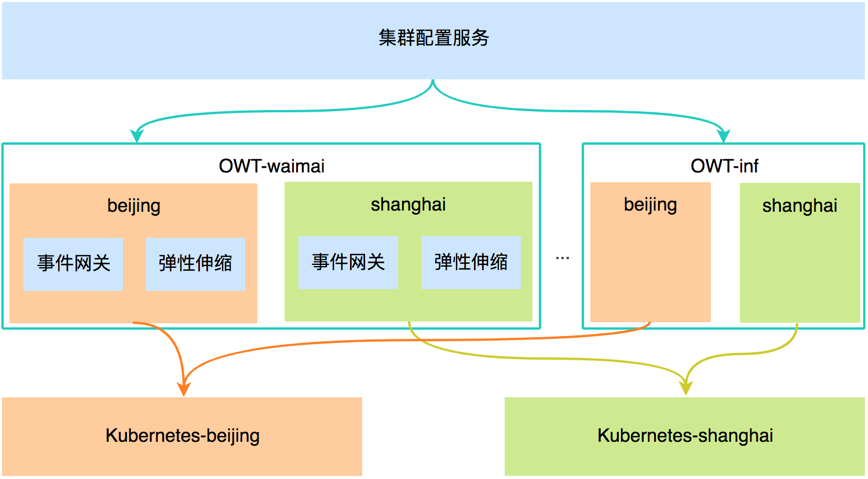
\includegraphics[width=0.7\linewidth]{images/nest_k8s_arch.png}
    \caption{美团Nest的部署架构}
    \label{nest_deploy_arch}
\end{figure}

对于规模更大的公有云例如AWS,
采取的是分地域+可用区的方式,
一方面实现隔离和高可用,
另一方面可以就近服务而提升性能\cite{aws_global_infra}。

\subsection{并发度限制}
尽管理论上Serverless具有无限的扩容能力,
但主流的Serverless平台都会进行并发限制,
通常有设置并发度的选项。
AWS默认每个区域为1000QPS
\footnote{AWS的并发限制是可以申请增加的,不设定上限,但需要提前申请。}\cite{lambda_concurrency};
Google Cloud Run单个容器默认限制为80,最高可设置为1000\cite{google_cloud_run_concurrency};
美团在事件网关上进行限流,
并支持对后端函数进行降级和限流\cite{meituan_serverless_nest}。

\subsection{关键服务高可用}
除了运行计算任务的集群本身需要进行分区外,
从系统架构上还需要对关键的服务进行高可用设计,
例如AWS Lambda的架构中,
最开始是不同的分区有单独的Worker Manager服务负责管理这个分区下的任务分配,
但由此带来的问题是一旦该服务出现问题会影响到整个分区,
因此Lambda在其最新的架构中引入了高可用的Assignment Service,
采用分布式共识算法来解决这一问题,
如\cref{lambda_assignment_service}所示。

\begin{figure}[ht!]
    \centering
    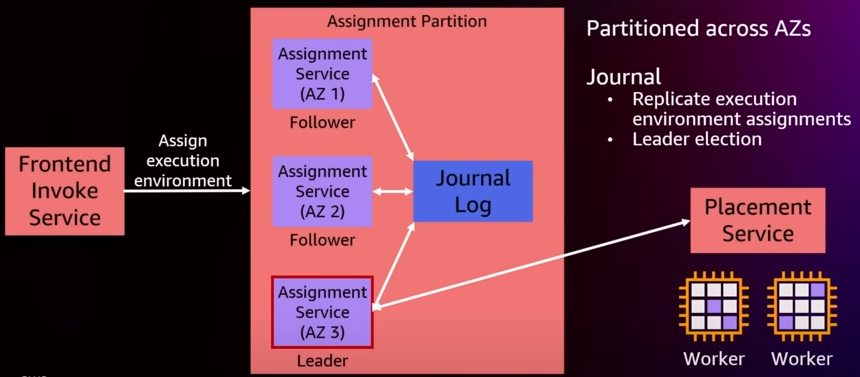
\includegraphics[width=\linewidth]{images/lambda_assignment_service.png}
    \caption{AWS Lambda架构中Assignment Service的高可用设计\cite{aws_lambda_2022}}
    \label{lambda_assignment_service}
\end{figure}